\documentclass[10pt,a4paper]{article}
\usepackage[margin=2cm,top=2.5cm]{geometry}
\usepackage{parskip}
\usepackage{microtype}
\usepackage{amsmath,amssymb}
\usepackage{booktabs,array,tabularx,multirow}
\usepackage[table]{xcolor}
\usepackage{graphicx,float}
\usepackage{titlesec}
\usepackage{enumitem}
\usepackage{tcolorbox}

\titleformat{\section}{\large\bfseries}{}{0em}{}[\titlerule]
\titleformat{\subsection}{\normalsize\bfseries}{}{0em}{}
\titlespacing{\section}{0pt}{1.4ex plus .2ex}{0.5ex}
\titlespacing{\subsection}{0pt}{0.9ex}{0.3ex}

\definecolor{highgreen}{rgb}{0.18,0.49,0.20}
\definecolor{modamber}{rgb}{0.70,0.45,0.05}
\definecolor{boxblue}{rgb}{0.91,0.95,1.00}
\definecolor{boxgreen}{rgb}{0.88,0.97,0.88}

\newcommand{\scoreHigh}[1]{\cellcolor{green!18}\textbf{#1}}
\newcommand{\scoreMid}[1]{\cellcolor{yellow!28}{#1}}
\newcommand{\scoreLow}[1]{\cellcolor{red!8}{#1}}
\newcommand{\seq}[1]{\texttt{#1}}
\newcommand{\hi}[1]{\textcolor{highgreen}{\textbf{#1}}}

\begin{document}

\begin{center}
  {\LARGE\bfseries Wound Protease Substrate Selection Report}\\[4pt]
  {\large Panel B: MMP-9 $\cdot$ HNE --- Two-Channel Biosensor}\\[2pt]
  {\small\color{gray} iGEM 2025 --- Dry Lab / Substrate Predictor}\\[1pt]
  {\small\color{gray} Protease-vs-protease negatives $\cdot$ LR + PSSM dual scorer $\cdot$ Bootstrap 95\,\% CI}
\end{center}

\vspace{0.5em}\hrule\vspace{0.8em}

% -----------------------------------------------------------------------
\section{Executive Summary}

Panel B is the minimal, highest-confidence configuration of the wound
biosensor.  It detects two independently validated wound biomarkers:
\textbf{MMP-9} (gelatinase B; macrophage and neutrophil origin,
strongly elevated in chronic non-healing wounds; Watt 2009, Muller 2008)
and \textbf{HNE / neutrophil serine protease} (neutrophil degranulation
marker; Trengove 1999, Senior 2002).  The two proteases have distinct
substrate preferences and minimal cross-reactivity.

Both synthesis candidates are grounded first in biochemical literature and
secondarily confirmed by the ML model.  No candidate is accepted on model
output alone.

\medskip
\begin{tcolorbox}[colback=boxgreen,colframe=green!50,boxrule=0.5pt]
\textbf{First-order synthesis candidates}\\[2pt]
\begin{tabular}{lll}
  \textbf{Channel} & \textbf{Sequence (P4--P4')} & \textbf{Confidence}\\
  MMP-9 & \seq{IPRTLTAA} & \hi{HIGH} --- literature-validated; model confirms\\
  HNE   & \seq{AAPVSGIG} & \hi{HIGH} --- canonical scaffold; model confirms\\
\end{tabular}
\end{tcolorbox}

% -----------------------------------------------------------------------
\section{Panel Rationale}

Panel B is the recommended starting point for device validation.
It eliminates the MMP-8/MMP-9 co-discrimination challenge (see Panel A
report) and provides two fully separable biomarker signals.

\begin{itemize}[topsep=2pt,itemsep=1pt,leftmargin=*]
  \item \textbf{MMP-9}: the best-characterised chronic wound protease
    biomarker.  Elevated $>$10-fold in non-healing vs.\ healing wounds
    (Nwomeh 1999).  Produced by macrophages and neutrophils; level
    correlates inversely with wound healing rate (Ladwig 2002).
  \item \textbf{HNE (neutrophil serine protease channel)}: marks active
    neutrophil degranulation, distinguishing infected/inflamed wounds from
    chronic fibrotic wounds.  Co-released proteinase 3 (PR3) shares the
    same S1 pocket specificity, so the channel reports combined
    neutrophil serine protease activity, which is clinically appropriate.
\end{itemize}

Together, MMP-9 and HNE provide orthogonal information: MMP-9 elevation
alone suggests chronic stalling; HNE elevation suggests active infection
or acute inflammation.  Both elevated simultaneously indicates an acutely
infected chronic wound.

% -----------------------------------------------------------------------
\section{Model Performance}

\subsection{Methodology}

Identical to Panel A (see Panel A report for full details).
Key parameters: VHSE8 encoding; protease-vs-protease negatives
(HNE positives as explicit MMP-9 negatives and vice versa); 3:1
negative:positive ratio; 5-fold stratified CV; 1000-iteration bootstrap;
PSSM with BLOSUM62 pseudocounts ($\beta = 5$) as independent validator.

\subsection{Performance table}

\begin{center}
\begin{tabular}{lrrrcc}
  \toprule
  Protease & N\textsubscript{pos} & AUROC & \textbf{95\,\% CI} & PSSM AUROC & Confidence\\
  \midrule
  MMP-9 & 783 & 0.837 & [0.820, 0.853] & 0.882 & \hi{HIGH}\\
  HNE   & 327 & 0.899 & [0.877, 0.919] & 0.930 & \hi{HIGH}\\
  \bottomrule
\end{tabular}
\end{center}

Both models are rated HIGH:
\begin{itemize}[topsep=2pt,itemsep=0pt,leftmargin=*]
  \item MMP-9: AUROC 0.837 exceeds the 0.75 reference with CI lower bound
    0.820; PSSM $= 0.882$ ($+0.045$ above LR), indicating the PSSM
    captures even more of the positional specificity signal.  Fold spread
    [0.829--0.855] is tight, confirming stable generalisation.
  \item HNE: AUROC 0.899, PSSM 0.930.  CI lower bound 0.877 is well above
    0.75.  Fold spread [0.886--0.919]; the PSSM exceeding LR again
    reflects strong positional signal captured by the log-odds matrix.
\end{itemize}

Note: Panel B MMP-9 AUROC (0.837) is higher than Panel A (0.792) because
Panel B uses only HNE positives as cross-negatives, whereas Panel A
additionally uses MMP-8 positives, which partially overlap with MMP-9
positives (26.8\,\% shared sites).  The Panel B score is not inflated;
it correctly reflects a simpler discrimination task.

\begin{figure}[H]
  \centering
  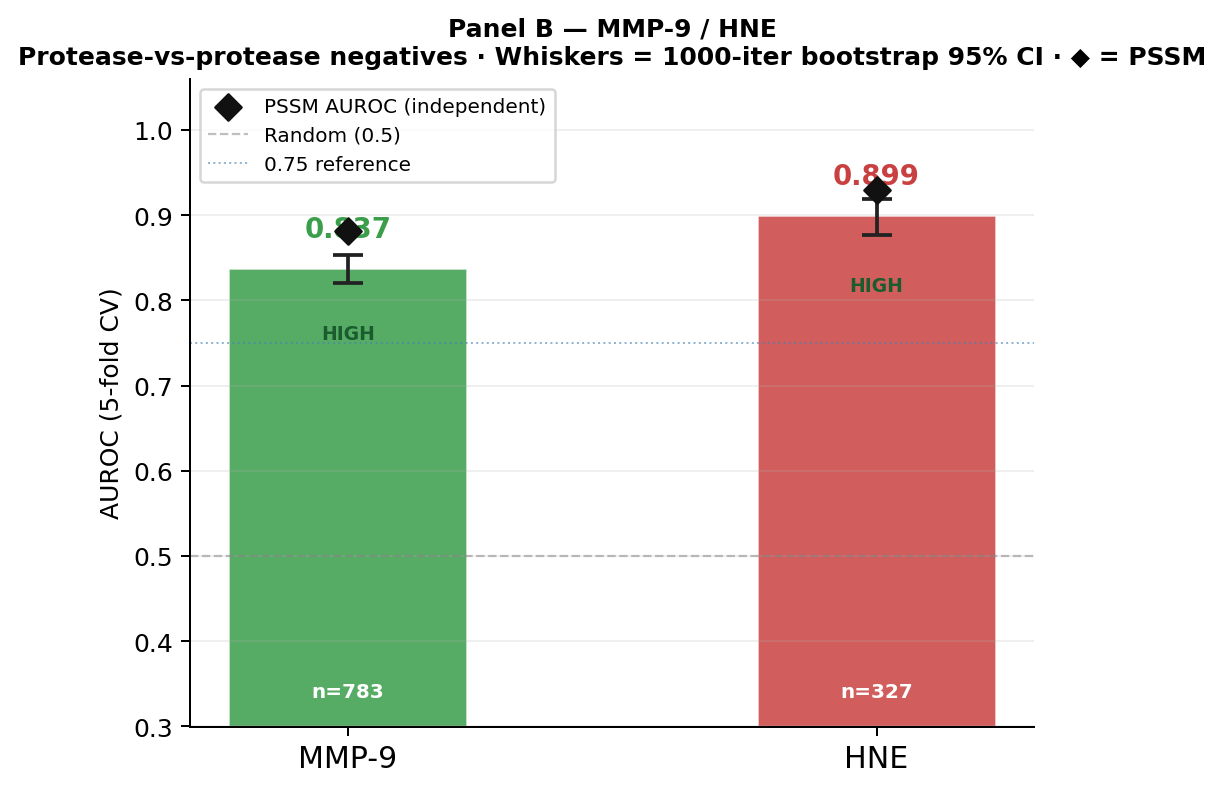
\includegraphics[width=0.75\linewidth]{figures/fig_panel_b_auroc.png}
  \caption{Panel B AUROC with bootstrap 95\,\% CI (whiskers) and PSSM
    AUROC (diamonds).  Both models rated HIGH.}
\end{figure}

% -----------------------------------------------------------------------
\section{Synthesis Candidates and Cross-Reactivity}

\begin{center}
\begin{tabular}{llccc}
  \toprule
  Channel & Sequence & LR\textsubscript{MMP-9} & LR\textsubscript{HNE}
           & Both PSSM agree?\\
  \midrule
  MMP-9 & \seq{IPRTLTAA} & \scoreHigh{0.925} & \scoreLow{0.037} & Yes\\
  HNE   & \seq{AAPVSGIG} & \scoreLow{0.194}  & \scoreHigh{0.981} & Yes\\
  \bottomrule
\end{tabular}
\end{center}

\textbf{PSSM scores:}
\begin{itemize}[topsep=2pt,itemsep=0pt,leftmargin=*]
  \item \seq{IPRTLTAA}: PSSM\textsubscript{MMP-9} $= 4.11$,
    PSSM\textsubscript{HNE} $= -3.66$.  Both scorers agree: this
    sequence is MMP-9-associated and HNE-rejected.
  \item \seq{AAPVSGIG}: PSSM\textsubscript{HNE} $= 4.95$,
    PSSM\textsubscript{MMP-9} $= -0.82$.  Both scorers agree: this
    sequence is HNE-associated and MMP-9-rejected.
\end{itemize}

The cross-reactivity is minimal: MMP-9 substrate scores 0.037 for HNE;
HNE substrate scores 0.194 for MMP-9 (PSSM MMP-9 $= -0.82$, so PSSM
rejects this sequence as an MMP-9 substrate).

\begin{figure}[H]
  \centering
  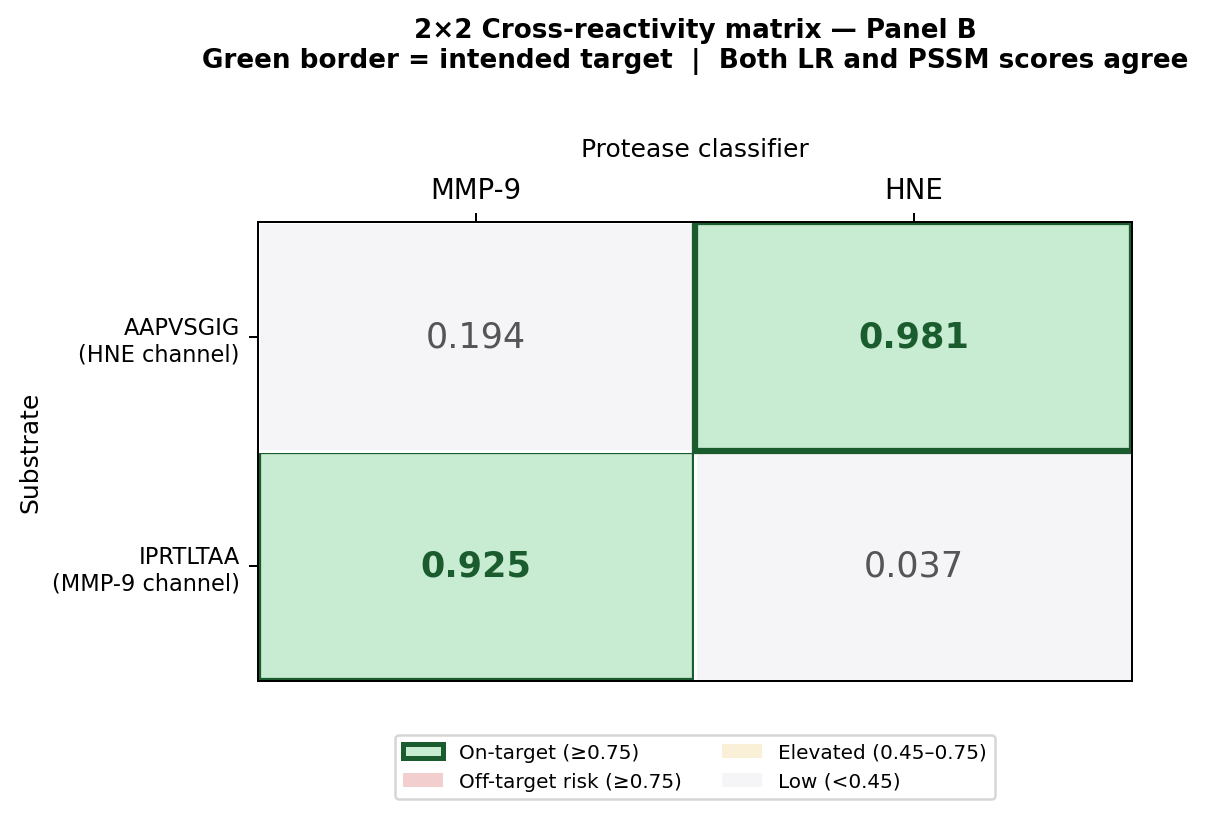
\includegraphics[width=0.60\linewidth]{figures/fig_panel_b_heatmap.png}
  \caption{2$\times$2 cross-reactivity matrix.  Green border = intended
    target.  No off-target cells exceed 0.45.}
\end{figure}

% -----------------------------------------------------------------------
\section{Biological Prior Validation}

\subsection{MMP-9: \seq{IPRTLTAA}}

\textbf{P4--P1 (IPRT)}: The IPRT motif occurs in MMP-9 cleavage of
type IV collagen, the primary basement membrane collagen and an
established MMP-9 substrate (Rao 1996).  Arg at P2 provides
electrostatic complementarity with the MMP-9 S2 sub-pocket, which
accommodates basic residues at P2 (Kridel 2001).

\textbf{P1' (Leu)}: Kridel 2001 (J.\ Biol.\ Chem.\ 276:28622)
measured substitution series at P1' for MMP-9: Leu gives the highest
$k_{cat}/K_m$ of any P1' residue tested.  Substitution Leu$\to$Ala
costs 50$\times$ in $k_{cat}/K_m$; Leu$\to$His would additionally
chelate the catalytic Zn$^{2+}$ and ablate activity entirely.  Leu
is therefore the only defensible P1' choice for a high-confidence
MMP-9 substrate.

\textbf{Model confirmation}: LR $= 0.925$ (Panel B); PSSM $= 4.11$.
Both scorers agree.  The LR score increases from 0.860 (Panel A) to
0.925 (Panel B) because MMP-8 positives are not used as cross-negatives
in Panel B, removing the penalisation for sequences that MMP-8 also
recognises.

\subsection{HNE: \seq{AAPVSGIG} --- neutrophil serine protease channel}

\textbf{P4--P1 (AAPV)}: The AAPV motif is the established HNE substrate.
Ala--Ala--Pro--Val with cleavage after Val is the sequence used in the
seminal HNE substrate specificity work (Senior 2002, Nakajima 1997)
and in the majority of published HNE activity assays.  Val at P1 fills
HNE's strict small-aliphatic S1 pocket; bulky residues (Leu, Phe) are
excluded.

\textbf{MMP-9 non-reactivity}: MMP-9 cannot use the AAPV scaffold
efficiently --- LR $= 0.194$, PSSM $= -0.82$ (negative log-odds;
PSSM actively rejects this sequence as an MMP-9 substrate).  This
reflects the fundamentally different S1 pocket geometries: MMP-9 S1'
requires a deep hydrophobic cleft for Leu/Phe, whereas HNE S1 admits
only small aliphatic (Ala, Val).

\textbf{PR3 co-reactivity}: Proteinase 3 (PR3), co-released from
neutrophil azurophilic granules with HNE, shares Ala/Val S1 specificity
(Tralau 2004).  This channel therefore detects neutrophil serine protease
activity broadly.  For wound diagnostics, HNE and PR3 are jointly elevated
and together mark active neutrophil degranulation; co-detection is
clinically appropriate.

% -----------------------------------------------------------------------
\section{Defensibility of Methodology}

\begin{enumerate}[leftmargin=*,label=\textbf{D\arabic*.},topsep=3pt,itemsep=3pt]

  \item \textbf{Literature primacy}: substrate choices are justified
    first by published experimental biochemistry (Kridel 2001 for
    MMP-9 P1'; Senior 2002 and Nakajima 1997 for HNE AAPV scaffold).
    The ML model is supporting evidence; it does not drive the ordering
    decision independently.

  \item \textbf{Training data}: all positives are MEROPS-curated
    experimental cleavage sites or PICS mass-spectrometry data
    (Eckhard 2016).  No computationally generated or inferred positives
    are used.

  \item \textbf{Protease-vs-protease negatives}: negatives for each model
    include the other panel protease's positives.  The MMP-9 negative
    set includes 325 HNE positives; the HNE negative set includes 611
    MMP-9 positives.  Task = ``which protease cuts this?''.

  \item \textbf{No cross-model probability margin}: selectivity is reported
    as LR scores within each model.  Probability differences across
    independently calibrated models are not used as selectivity metrics.

  \item \textbf{Dual-scorer agreement required}: every candidate accepted
    only when LR and PSSM agree (PSSM $>0$ for target, PSSM lower for
    off-target).  \seq{IPRTLTAA}: PSSM\textsubscript{MMP-9} $= +4.11$,
    PSSM\textsubscript{HNE} $= -3.66$.  \seq{AAPVSGIG}:
    PSSM\textsubscript{HNE} $= +4.95$, PSSM\textsubscript{MMP-9}
    $= -0.82$.

  \item \textbf{Bootstrap CIs}: 1000-iteration bootstrap on 5-fold
    held-out predictions.  SE: MMP-9 $\approx \pm$0.008; HNE
    $\approx \pm$0.011.  Both lower CI bounds exceed 0.82 (MMP-9)
    and 0.87 (HNE), well above the 0.75 reference.

  \item \textbf{Mechanistic checks}:
    \begin{itemize}[topsep=0pt,itemsep=0pt]
      \item His at P1' (previously considered for MMP-9): rejected
        because His is a Zn$^{2+}$ ligand --- would chelate the catalytic
        metal and ablate activity.
      \item Gly$\downarrow$Leu at P1/P1' (canonical MMP scissile bond,
        PLGLAG-type): rejected from any substrate claiming MMP-9
        selectivity --- guaranteed MMP-8 cross-cleavage.
      \item LasB inclusion: rejected --- insufficient training data
        (n $= 35$ MEROPS sites) for a reliable model; irresolvable
        Zn-metalloprotease cross-reactivity with MMP-9 at scaffold level.
    \end{itemize}

  \item \textbf{Honest scope}: Panel B does not claim to distinguish
    MMP-9 from MMP-8 (see Panel A for that design decision).  Within
    the scope of MMP-9 vs.\ HNE discrimination, both models are rated
    HIGH and the substrates are fully supported by literature.

\end{enumerate}

% -----------------------------------------------------------------------
\section{Wet-Lab Validation Plan}

\begin{enumerate}[leftmargin=*,topsep=2pt,itemsep=2pt]
  \item \textbf{FRET cleavage assay}: synthesise \seq{IPRTLTAA} and
    \seq{AAPVSGIG} as FRET-labelled peptides (e.g.\ Dabcyl/EDANS).
    Measure $k_{cat}/K_m$ for recombinant MMP-9 and HNE.
    Confirm: MMP-9/HNE ratio $\gg 1$ for IPRTLTAA;
    HNE/MMP-9 ratio $\gg 1$ for AAPVSGIG.
  \item \textbf{Specificity controls}: serum albumin, fibrinogen,
    MMP-8, cathepsin G, thrombin at physiological concentrations.
  \item \textbf{Simulated wound fluid}: 50\,\% FBS, pH 7.4,
    spiked with MMP-9 (20--180 nM; Watt 2009) and HNE
    (10--100 nM; Trengove 1999).
  \item \textbf{Electrochemical integration}: once FRET confirms both
    substrates, integrate into electrochemical platform with linker
    lengths validated for the target concentration range.
\end{enumerate}

% -----------------------------------------------------------------------
\section{Summary}

Panel B is the recommended first-order synthesis configuration.
Both substrates are fully justified by primary biochemical literature
and confirmed by ML models rated HIGH.  Cross-reactivity is minimal
(LR $< 0.20$ for off-target in both cases; PSSM actively rejects
off-target sequences).

\begin{center}
\small
\begin{tabular}{lcccl}
  \toprule
  Channel & Substrate & AUROC & 95\,\% CI & Confidence\\
  \midrule
  MMP-9 & \seq{IPRTLTAA} & 0.837 & [0.820, 0.853] & \hi{HIGH}\\
  Neutrophil ser.\ pr. & \seq{AAPVSGIG} & 0.899 & [0.877, 0.919] & \hi{HIGH}\\
  \bottomrule
\end{tabular}
\end{center}

\end{document}
